\documentclass[aps,prd,twocolumn,10pt,superscriptaddress,nofootinbib,longbibliography,floatfix]{revtex4-2}

\usepackage{amsmath,amssymb,amsfonts}
\usepackage{bm}
\usepackage{graphicx}
\usepackage{booktabs}
\usepackage{xcolor}
\usepackage{hyperref}
\graphicspath{{figures/}}
\hypersetup{colorlinks=true,linkcolor=blue,citecolor=blue,urlcolor=blue}

\newcommand{\dd}{\mathrm{d}}
\newcommand{\Mpl}{M_\mathrm{Pl}}
\newcommand{\Ham}{\mathcal{H}}
\newcommand{\Mom}{\mathcal{M}}
% a result of work still in progress goes where this marker stands
\newcommand{\pending}[1]{\textcolor{red}{[Pending: #1]}}

\begin{document}

\title{Stochastic inflation in numerical relativity:\\ Specification, feasibility and the slow-roll reproduction (working note v1)}

\author{Track E of the numerical-relativity particle-in-cell cosmology program}

\date{Working note v1, state of 21 November 2026}

\begin{abstract}
The abundance of primordial black holes is set by the rare, large curvature perturbations of inflation, and the standard tool for their statistics, stochastic delta N, rests on a separate-universe approximation whose validity at sudden transitions to ultra-slow roll is disputed. Launay, Rigopoulos and Shellard added the quantum noise to the full Einstein--scalar-field equations as stochastic sources and evolved one slow-roll and one ultra-slow-roll case. This working note records the reproduction of those cases in the numerical-relativity code of this program, as the first step towards tail statistics computed without the separate-universe approximation. At the feasibility gate it fixed the equations, the coarse-graining window, the gauge, the initial slice and acceptance criteria that a single realization can pass or fail, corrected the source papers where needed, provided reference solutions for the freezing of super-horizon modes and for stochastic delta N, and validated the noise generator of the code. In the slow-roll case the code now reproduces linear theory mode by mode on lattices up to the size of the source paper: every resolved mode follows its linear solution with the same random number far inside the tolerance, and every mode that left the window early enough freezes as linear theory with metric perturbations predicts, which excludes a lattice on a fixed background by a wide margin. The constraint violation consists of the expected part of second order in the noise, independent of the resolution, and a part of first order that the difference stencils produce when the shortest modes enter with four cells per wavelength. That part converges with resolution, but it fails the track's strict criterion in the source paper's set-up, a failure kept on record. One realization costs far less than the threshold at which the track would be downgraded.
\end{abstract}

\maketitle

\section{Introduction}\label{sec:intro}

Primordial black holes form where the comoving curvature perturbation of inflation is large enough for a region to collapse once it re-enters the Hubble radius. Their abundance therefore depends on the far tail of the distribution of the curvature perturbation, many standard deviations away from the mean. In models where the inflaton crosses a nearly flat stretch of its potential, a phase of ultra-slow roll (USR) amplifies the perturbations on the scales that leave the Hubble radius during it, and quantum diffusion of the field dominates over its classical drift. Stochastic inflation describes this diffusion: the long-wavelength part of the field obeys a Langevin equation driven by the short-wavelength modes that cross a coarse-graining scale, and the stochastic delta-N formalism converts the distribution of first-passage times into the distribution of the curvature perturbation \cite{Fujita:2013alg,Jackson:2022is}. Applied to USR, it has been used to compute the distribution of the compaction function that decides collapse \cite{Raatikainen:2023cf,Raatikainen:2025kicks}.

Stochastic delta N evolves each coarse-grained patch as a separate homogeneous universe. This separate-universe approximation is disputed at the sudden transitions into and out of USR \cite{Jackson:2023su}. Lattice simulations of the field on a fixed expanding background keep the gradients \cite{Caravano:2024usr}; without metric perturbations, however, the super-horizon curvature perturbation fails to freeze, and its power decays even in slow roll \cite{Barker:2026lattice}. Launay, Rigopoulos and Shellard therefore added the stochastic sources to the full Einstein--scalar-field system in its 3+1 form \cite{Launay:2024sigr}, built Bunch--Davies initial data for numerical relativity \cite{Launay:2025bd}, and evolved a slow-roll (SR) and a USR case with a BSSN code \cite{Launay:2025sinr}; the thesis of Launay collects the material with corrections \cite{Launay:2026thesis}. Their tests use one realization per case. Large samples, tail statistics and the hand-over to black-hole formation are open.

This program applies a version of the numerical-relativity particle-in-cell code of Wu and Most \cite{Wu:2026nrpic}, built in AthenaK \cite{Stone:2024athenak}, to cosmology. Its Track E asks whether the same code, extended with a scalar field and the stochastic sources, reproduces the two cases of Ref.~\cite{Launay:2025sinr} at an affordable cost per realization; only then do tail statistics in full general relativity become a realistic goal. The work is carried out by large-language-model agents under human direction. This note records the feasibility gate and the slow-roll gate: (i) a specification of the reproduction with acceptance criteria, including a freezing test per Fourier mode (Sec.~\ref{sec:problem}); (ii) the set-up in the code and the corrected initial slice (Sec.~\ref{sec:setup}); (iii) reference solutions for the freezing of super-horizon modes and for stochastic delta N, and the validation of the code's noise generator (Sec.~\ref{sec:tests}); (iv) the cost of one realization and the decision of the feasibility gate (Sec.~\ref{sec:cost}); (v) the slow-roll reproduction: background, amplitude of every mode, freezing and order in time (Sec.~\ref{sec:sr}); (vi) the constraints, their parts of first and second order in the noise, and the criterion that judges them (Sec.~\ref{sec:constraints}); (vii) the validation of the analysis, the reproducibility of the runs and the measured cost (Sec.~\ref{sec:validation}).
Section~\ref{sec:open} lists what is open. The parameters are in Appendix~\ref{app:parameters}, the corrections to the source papers in Appendix~\ref{app:errata}, and every number with the registered run that produced it in Appendix~\ref{app:ledger}.

\section{The problem and the test cases}\label{sec:problem}

\subsection{Stochastic sources in the Einstein--scalar-field equations}\label{sec:sources}

The quantum modes of the inflaton become classical once they are stretched beyond the Hubble radius. Stochastic inflation keeps the long-wavelength part of the fields as the evolved variables and adds, as a source, the modes that cross a coarse-graining scale $k_\sigma=\sigma aH$ at each moment, where $a$ is the scale factor, $H$ the Hubble rate and $\sigma$ a parameter of order one. Following Ref.~\cite{Launay:2025sinr}, the crossing is smoothed by the window
\begin{equation}\label{eq:window}
W_k(t)=\tfrac12\left\{1+\tanh\!\left[s\,\ln\frac{k_\sigma(t)}{k}\right]\right\},
\end{equation}
with steepness $s$. Every source derives from the linear comoving curvature perturbation $\mathcal{R}_k(t)\,\alpha_{\bm k}$, where $\mathcal{R}_k$ is the mode function of the Mukhanov--Sasaki equation and $\alpha_{\bm k}$ a complex unit Gaussian drawn once per wave vector. In e-folds $N$ the mode equation reads
\begin{equation}\label{eq:ms}
\mathcal{R}_k''+(3-\epsilon_1-\epsilon_2)\,\mathcal{R}_k'+\left(\frac{k}{aH}\right)^2\mathcal{R}_k=0,
\end{equation}
with the slow-roll parameters $\epsilon_1=-\dd\ln H/\dd N$ and $\epsilon_2=-\dd\ln\epsilon_1/\dd N$ in the sign convention of the source papers, so that $\epsilon_2=6$ in exact USR. The dimensionless power of a mode is $\Delta_\mathcal{R}=k^3|\mathcal{R}_k|^2/(2\pi^2)$. The curvature source is
\begin{equation}\label{eq:SR}
S_\mathcal{R}=\left\{\mathcal{R}_k\ddot W_k+\left[2\dot{\mathcal{R}}_k+(3-\epsilon_2)H\mathcal{R}_k\right]\dot W_k\right\}\alpha_{\bm k},
\end{equation}
and all field sources follow from it through the linear dictionary of the coarse-grained perturbations \cite{Launay:2024sigr,Launay:2025sinr}:
\begin{equation}\label{eq:sources}
\begin{aligned}
S_\Pi&=\sqrt{2\epsilon_1}\,\Mpl\,S_\mathcal{R},\qquad S_K=-\epsilon_1S_\mathcal{R},\\
S_{\tilde A_{ij}}&=\epsilon_1\left(\frac{\delta_{ij}}{3}-\frac{k_ik_j}{k^2}\right)S_\mathcal{R},
\end{aligned}
\end{equation}
for the momentum $\Pi$ of the scalar field $\phi$, the trace $K$ of the extrinsic curvature and its conformal trace-free part $\tilde A_{ij}$. The conformal metric, the conformal factor and the constraints carry no source; the constraints are then satisfied up to second order in the noise. These are the stochastic sources. Their coefficients can be taken from the Friedmann background (level 0 of the stochastic backreaction), from box means (level 1) or from local values (level 2) \cite{Launay:2025sinr}.

\subsection{The two test cases}\label{sec:cases}

The SR case is the quadratic potential $\tfrac12m^2\phi^2$ on its attractor; the USR case is the Higgs-like potential with a stationary inflection point of Ref.~\cite{Launay:2025sinr}, in which the field rolls onto the flat stretch and its velocity decays as $a^{-3}$ until it has crossed it. The simulation starts $N_*-N_0$ e-folds after the Bunch--Davies time $N_0$ of the mode functions and lasts until $N_f$; the box is periodic with $256$ cells per side, its size is chosen so that the longest mode enters the window at the start, and the noise reaches up to $k_\mathrm{max}=64\,\Delta k$, half the Nyquist wave number. Figure~\ref{fig:background} shows the background of both cases as computed by the reference integrator of the track, and Table~\ref{tab:parameters} lists the parameters. Over the run of the USR case the first slow-roll parameter falls by about ten orders of magnitude, while the modes enter the window during the first four e-folds, partly before and partly during USR.

\begin{figure*}
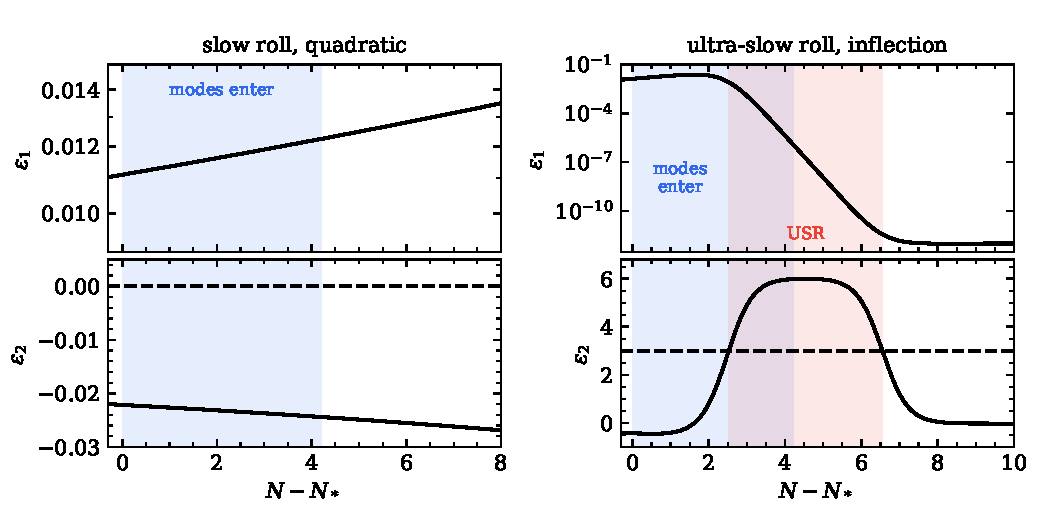
\includegraphics[width=\textwidth]{fig_background}
\caption{Background of the two test cases against the e-folds since the start of the simulation. Top: first slow-roll parameter; bottom: second, in the convention of the source papers (dashed: zero, and the USR threshold three). Blue band: the lattice modes enter the noise window; red band: ultra-slow roll.}
\label{fig:background}
\end{figure*}

\subsection{Acceptance criteria}\label{sec:criteria}

Reference~\cite{Launay:2025sinr} reports agreement of its spectra with linear theory in words. The reproduction fixes criteria that a single realization can pass or fail, because the code and the reference share the Gaussian numbers $\alpha_{\bm k}$ of each wave vector. Its central criterion concerns freezing. Without metric perturbations the Mukhanov--Sasaki equation acquires an extra term \cite{Barker:2026lattice}, and in slow roll a super-horizon mode then decays as
\begin{equation}\label{eq:decay}
\frac{\dd\ln\Delta_\mathcal{R}}{\dd N}=-4\epsilon_1,
\end{equation}
since $\mathcal{R}^2$ follows $H^4$. With metric perturbations the gradient correction decays as $e^{-2(N-N_k)}$ after the mode crosses the window at $N_k$, and the mode freezes. The freezing criterion compares, for every lattice mode that left the window at least six e-folds before the end, the measured power ratio between $N_k+4$ and $N_f$ with the same ratio of the full Mukhanov--Sasaki solution; the deformed equation of the fixed-background lattice misses it by about twenty times the tolerance. In USR only the longest modes discriminate, and there the comparison is with the full solution at the end of the run. The further criteria are: the box means of the background, the power of each mode against $W_k\mathcal{R}_k\alpha_{\bm k}$ for modes up to half the noise cutoff, second-order constraint violations with a sign-flipped source as negative control, convergence in space at the order of the stencils and in time at the order of the integrator, and bit-identical noise across domain decompositions and restarts. They carry the labels A1--A7; A8 compares one-point statistics with stochastic delta N. Their tolerances are fixed in the track's scoping text.

\section{Set-up and numerical methods}\label{sec:setup}

\subsection{The calculation in the code}\label{sec:code}

Figure~\ref{fig:architecture} shows the calculation in four states. The evolution runs in the program's AthenaK: the Z4c system with the constraint-damping variable switched off, which is BSSN, in geodesic slicing with zero shift on a periodic mesh; a minimally coupled scalar field whose stress--energy enters the spacetime solver; and the stochastic hook, which advances the mode functions of every lattice wave vector together with the field, synthesizes the source fields and adds them to the right-hand sides of $\Pi$, $K$ and $\tilde A_{ij}$. The release of the code at the feasibility gate contained these parts. The two releases since then add the initial slice at the start, with the mode tables of both cases; a record of the constraints and their term magnitudes at every step; dumps of the fields and the metric in double precision; and a linear model of the code's difference equations for each wave vector. The track supplies the references, the reconstruction of the curvature perturbation from the evolved fields, the per-mode criteria and the split of the constraints into parts odd and even in the noise amplitude (Sec.~\ref{sec:sr}). The box-mean coefficients (level 1) exist in other parts of the code and have to be carried over. Level 2 is left for later; Ref.~\cite{Launay:2025sinr} reports that switching it off changes the spectrum by a small fraction, and the reproduction states the difference.

\begin{figure*}
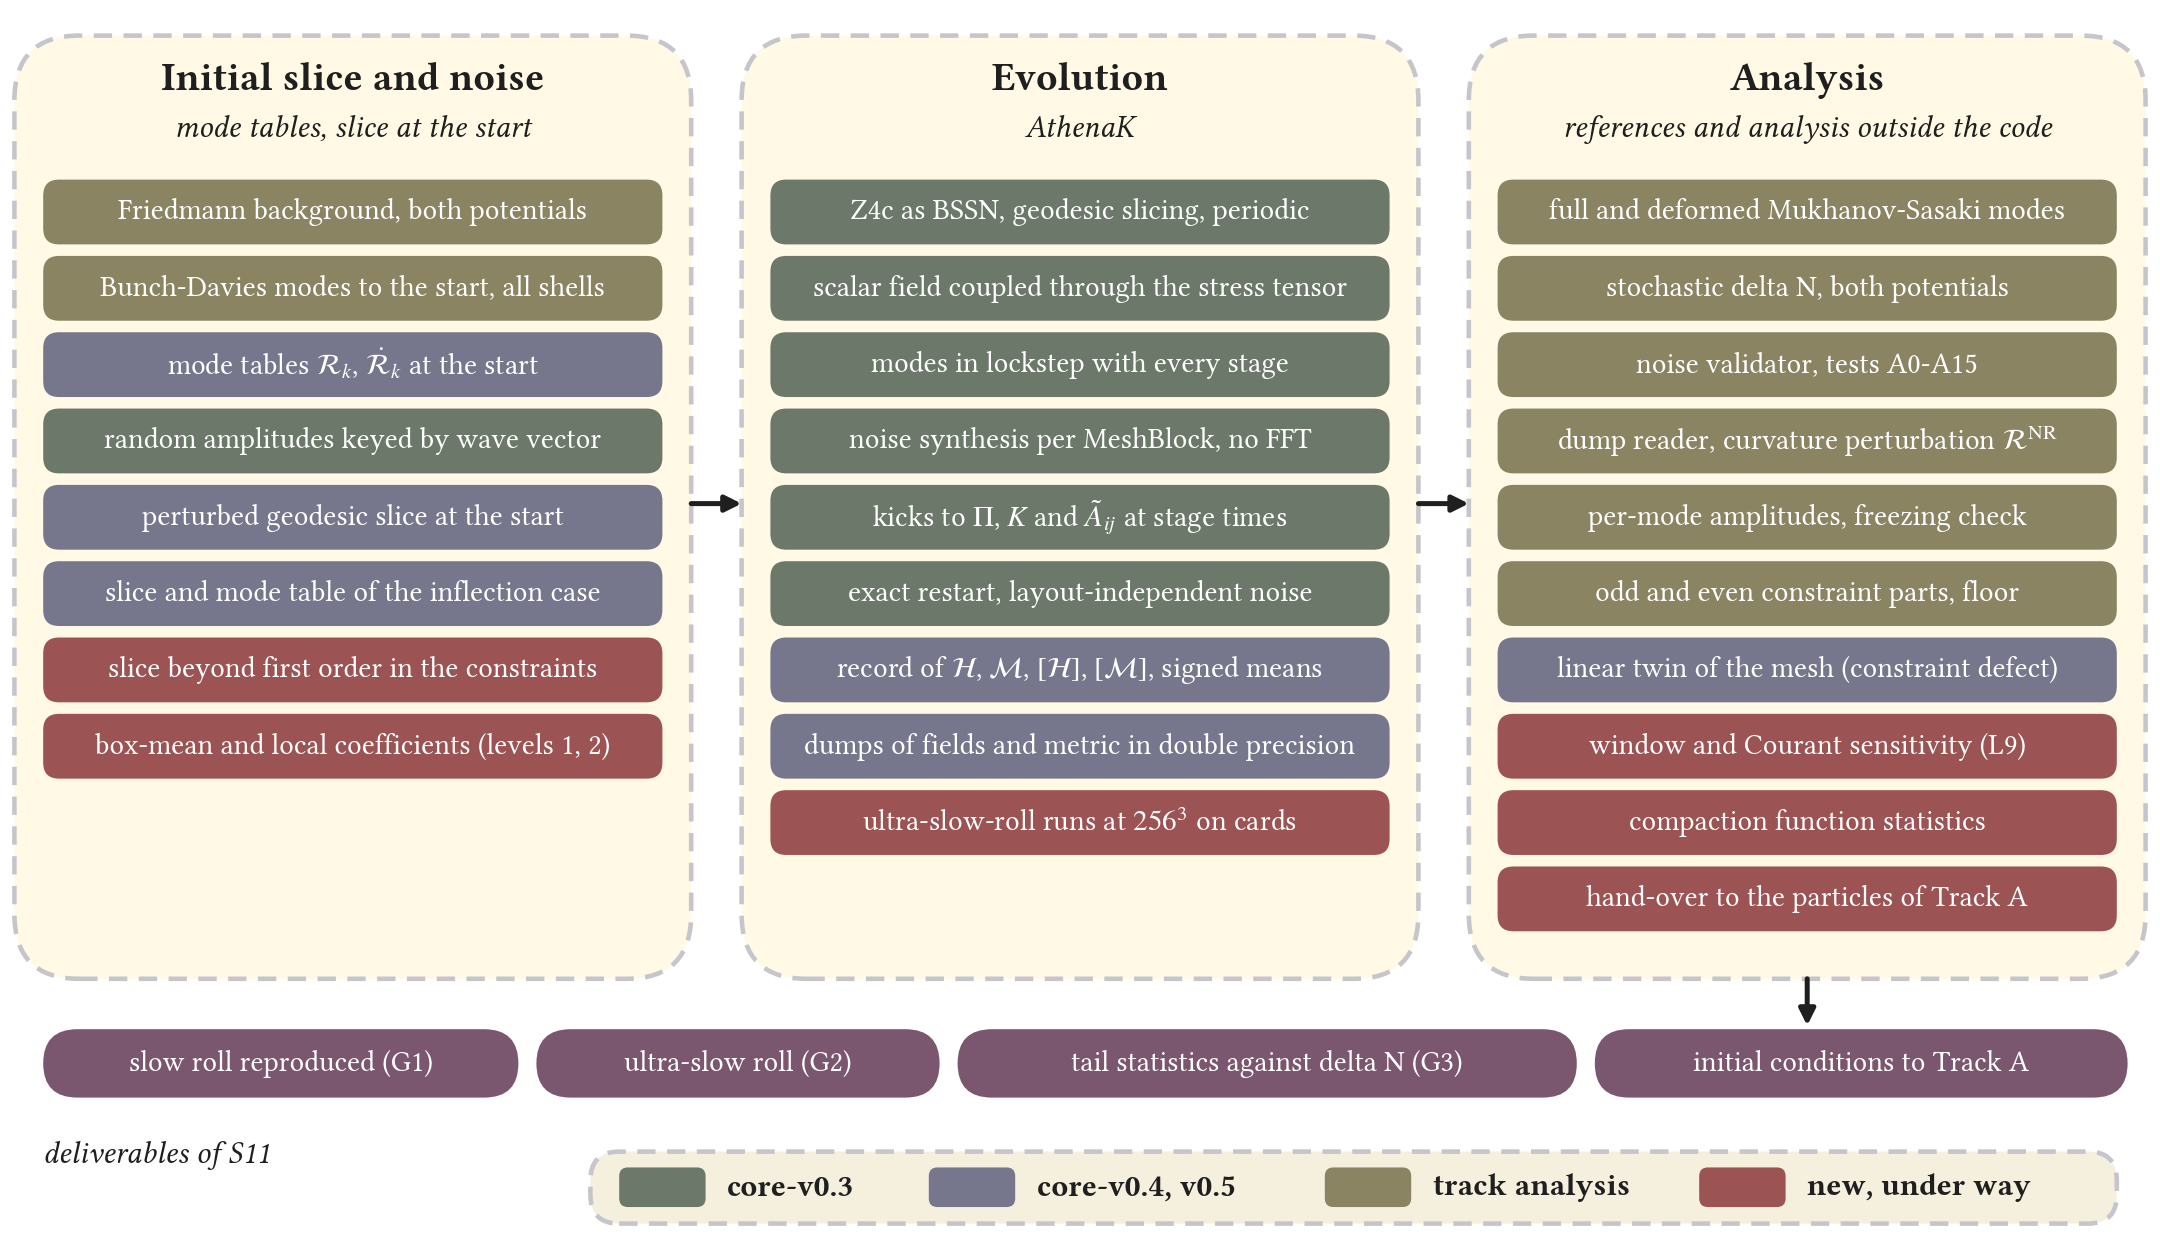
\includegraphics[width=0.92\textwidth]{schem_architecture}
\caption{Architecture of the track's calculation. Left: what the run starts from; centre: the evolution in AthenaK; right: references and analysis outside the code. Colours mark what the release of the code at the feasibility gate contained, what the two later releases added, what the track's analysis provides, and what is new or under way; the purple pills are the deliverables of the track.}
\label{fig:architecture}
\end{figure*}

\subsection{The noise}\label{sec:noise}

The code draws $\alpha_{\bm k}$ from a counter-based generator keyed by the wave vector, so the same realization appears at every resolution and in every decomposition of the mesh into blocks, and it synthesizes the real-space source on each block as a separable sum over the modes, without a Fourier library. The source papers integrate the window over each step with the mode functions frozen and treat the result as a Stratonovich increment. With the Gaussian numbers drawn once and a smooth window, the source of each realization is a smooth function of time; the code therefore evaluates it at the time of each Runge--Kutta stage, with the window derivatives in closed form, and the integrator keeps its order. Three noise schemes exist for tests: the frozen draw above, and two Markov schemes that draw new numbers in every step with a smooth or a step-like window.

\subsection{The initial slice}\label{sec:slice}

At the start the fields carry the coarse-grained linear perturbation $W\mathcal{R}$ in geodesic slicing, with the residual gauge freedom fixed as in Ref.~\cite{Launay:2025bd}. In terms of the Bardeen potential $\Phi_B=\Psi_B=-\epsilon_1Ha^2k^{-2}\dot{\mathcal{R}}$ the momentum perturbation of the field is
\begin{equation}\label{eq:dPi}
\begin{split}
\delta\Pi={}&\sqrt{2\epsilon_1}\,\Mpl\left(\dot{\mathcal{R}}-\dot\Phi_B-H\Psi_B\right)\\
&-\epsilon_2\sqrt{\epsilon_1/2}\;H\Mpl\left(\mathcal{R}-\Phi_B\right).
\end{split}
\end{equation}
The printed initial data of Ref.~\cite{Launay:2025bd} carry, in place of the $H\Psi_B$ term, a term in the lapse potential of the geodesic gauge, which vanishes there; with the printed form the linearized Hamiltonian constraint is violated at first order, with the form above it holds identically. The term follows from the gauge dictionary of the same paper once the time derivative of the gauge shift is kept. This is the corrected momentum of the initial slice; Appendix~\ref{app:errata} lists it with the other corrections.

\subsection{Numerical methods}\label{sec:methods}

Spatial derivatives are centred sixth-order differences, matching Ref.~\cite{Launay:2025sinr}; Kreiss--Oliger dissipation and constraint damping are off. Time integration is the low-storage fourth-order Runge--Kutta scheme of the code, and the mode functions are advanced with the same stage coefficients, so that each stage evaluates its sources at its own time. With Courant factor $\theta$ the number of steps is
\begin{equation}\label{eq:steps}
N_T=\frac{N\sigma\,\Delta N}{2\pi\theta},
\end{equation}
for $N$ cells per side and $\Delta N$ e-folds \cite{Launay:2025sinr}; the reproduction uses $\theta=0.25$ and tests one half and one quarter of it. The reference solutions outside the code are ordinary differential equations: the background and the full and deformed Mukhanov--Sasaki equations for every lattice shell from Bunch--Davies data, solved by two independent integrators, and a phase-space Langevin solver with first-passage detection for stochastic delta N.

\section{Reference solutions and tests}\label{sec:tests}

\subsection{Freezing of super-horizon modes}\label{sec:freezing}

Figure~\ref{fig:freezing} is the reference for the freezing criterion. With metric perturbations, the power of every slow-roll mode approaches its final value within a few e-folds of crossing and stays there, slightly above the slow-roll estimate at crossing; after four e-folds the remaining drift is far below the tolerance. The deformed equation decays at the rate four times the first slow-roll parameter, integrated along the background, for all modes alike, and ends a third below the full power for the longest mode. In USR the two equations differ only for the modes that crossed the window about an e-fold or more before the onset of USR: there the deformed power at the end exceeds the full one by up to a factor of eight, and from about ten lattice spacings on the two agree closely. A second, independent integration of one mode per case reproduces these slopes and ratios.

\begin{figure}
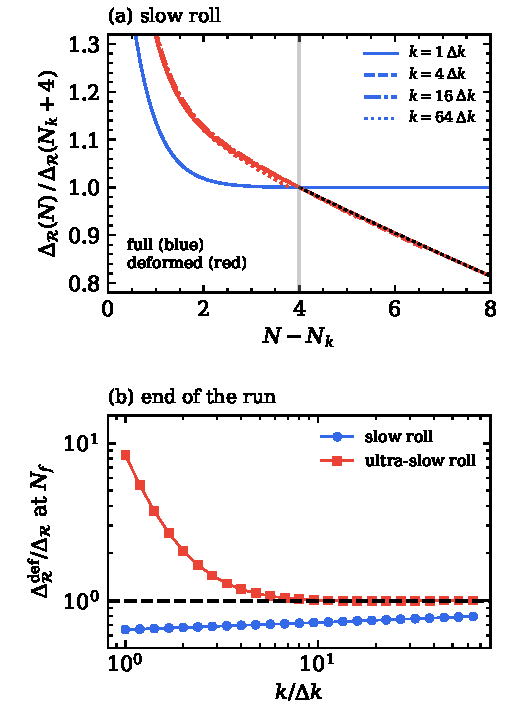
\includegraphics[width=\columnwidth]{fig_freezing}
\caption{Freezing of super-horizon modes. (a) Slow roll: power of four modes, divided by its value four e-folds after the mode crossed the window scale, with metric perturbations (blue) and without (red); dotted: the decay rate of the deformed equation. (b) Deformed over full power at the end of the run, for every lattice shell.}
\label{fig:freezing}
\end{figure}

\subsection{Stochastic delta N for the same potentials}\label{sec:deltaN}

The comparison outside numerical relativity evolves the background field and its velocity under the noise of the same lattice band, with the noise covariance taken from the linear modes, and measures the number of e-folds to a surface of uniform field fifteen e-folds after the start. The Langevin solver reproduces the analytic first-passage moments of the drift--diffusion problem and the closed-form distribution of quadratic inflation \cite{Fujita:2013alg,Jackson:2022is}. Figure~\ref{fig:deltan} shows the result for both potentials. With a narrow window, $\sigma=0.01$, the variance equals the linear variance of the band and the distribution is Gaussian to four standard deviations in slow roll, with a small positive skewness in USR. With $\sigma=1$, the coarse-graining of the numerical-relativity runs, the variance exceeds the linear value by more than two fifths in both cases, because a mode handed to the separate universe at Hubble crossing still carries gradient energy: evolved without gradients, a massless mode ends at $13/9$ of its frozen power. Criterion A8 therefore compares the one-point statistics of the numerical-relativity runs with the $\sigma=0.01$ reference and with the lattice sum of the band, which in slow roll exceeds the continuum integral (dotted line).

\begin{figure}
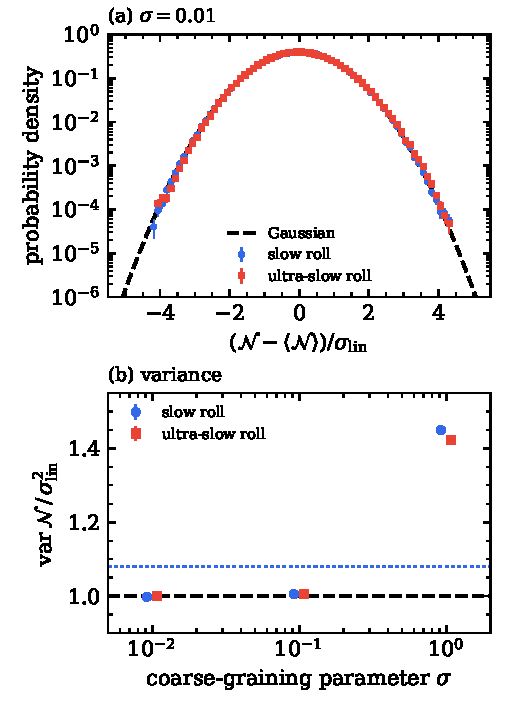
\includegraphics[width=\columnwidth]{fig_deltan}
\caption{Stochastic delta N for the two test cases. (a) Distribution of the number of e-folds about its mean, in units of the linear standard deviation of the noise band, for $\sigma=0.01$; dashed: unit Gaussian. (b) Variance over the linear variance against the coarse-graining parameter; dotted: lattice sum of the band in slow roll.}
\label{fig:deltan}
\end{figure}

\subsection{Reproducible noise in the code}\label{sec:noisetest}

Before the code existed, the track wrote the noise contract: sixteen tests on the dumped source fields, from the exact reconstruction of each field from its keys, through the spectrum per shell, Gaussianity, correlations and the band limit, to bit-identity across MeshBlock layouts and restarts and independence of seeds. A self-test with planted errors confirmed that the validator catches each kind of error. Figure~\ref{fig:noise} shows the validation of the code's generator, built from the scalar-field branch before the release, in a scaled base case on processors. The frozen scheme passes every test, with the fields bit-identical for one, eight and sixty-four MeshBlocks and through a restart, and the same coefficients at two resolutions to rounding error. The Markov scheme with a step window passes every applicable test. The Markov scheme with the smooth window passes all tests except the exact reconstruction, which it misses by an order of magnitude: for modes long past crossing the window increment is a difference of two numbers close to one, and the code and the reference evaluate the window with different math libraries. Modes still entering agree to rounding error. The frozen draw, which the reproduction uses, involves no such difference. The released code forms the increment of the smooth window as a quotient of hyperbolic functions; validated against a reference that forms it the same way, its Markov scheme with the smooth window passes every test, the reconstruction to rounding error (open diamonds), while the reference with the difference still misses the tolerance, so the remaining discrepancy sits in the reference.

\begin{figure}
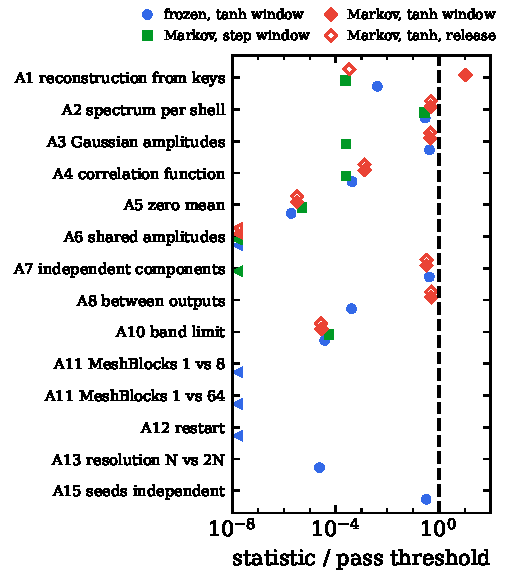
\includegraphics[width=\columnwidth]{fig_noise}
\caption{Validation of the code's noise generator for three noise schemes before the release, and for the Markov scheme with the smooth window of the released code (open diamonds). Each test statistic is divided by its pass threshold, so a test passes at or left of the dashed line; left-pointing markers at the edge are results that are exactly zero.}
\label{fig:noise}
\end{figure}

\subsection{Corrections to the source papers}\label{sec:errata}

The specification read the equations at their sources and checked them by independent derivation or by registered calculations. Besides the momentum of the initial slice (Sec.~\ref{sec:slice}), the printed prefactors of the random draw give too much power by powers of $2\pi$, the importance-sampling weight of Ref.~\cite{Jackson:2022is} carries a sign that moves its expectation far from unity, for a finite ultraviolet boundary the leading pole of the first-passage distribution is the lowest eigenvalue of the problem, in place of the value stated as leading in general, the Friedmann denominator of Ref.~\cite{Launay:2025sinr} lacks a factor, and the USR interval in its text lies about one e-fold later than in its own figure. The spectra and constraints that Refs.~\cite{Launay:2025bd,Launay:2025sinr} report agree with the corrected forms, so their codes presumably use them. Appendix~\ref{app:errata} lists the corrections.

\section{Cost and the decision at the feasibility gate}\label{sec:cost}

The scoping model priced one step from the measured throughput of the spacetime solver alone, plus an assumed overhead for the field and the sources and an assumed rate of the synthesis. The code's measured throughput on one card, with the field and with the stochastic sources at the noise band of a $128^3$ box, replaces both assumptions: the overhead is about four times the assumed one. Scaling only the synthesis with its operation count to $256^3$, one realization of either case costs about one and a half times the scoping model, still far below the downgrade threshold of the track (Fig.~\ref{fig:cost}). The two production runs and the convergence ladder to the USR gate then fit in the allotment of the track several times over. A thousand realizations for tail statistics would cost several hundred card-hours; that scope is decided at the USR gate.

\begin{figure}
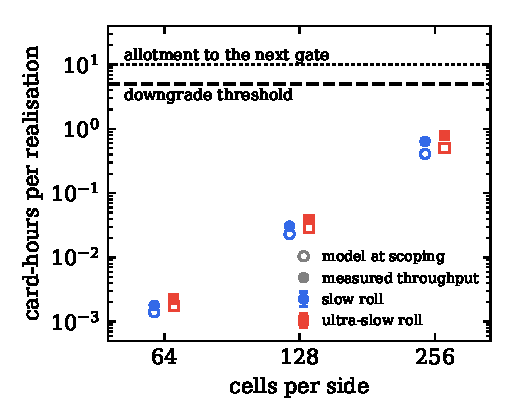
\includegraphics[width=\columnwidth]{fig_cost}
\caption{Card-hours of one realization against the number of cells per side, at Courant factor one quarter. Open markers: the model at scoping; filled markers: the same step counts with the measured throughput of the code (bars: the range of block sizes at $256^3$). Dashed: downgrade threshold; dotted: allotment to the next gate.}
\label{fig:cost}
\end{figure}

The feasibility gate asked the group to continue, to shrink or to downgrade. The specification was complete, the implementation existed in the code the program chose, its noise generator passed the contract in the scheme the reproduction uses, and the cost was affordable; the track recommended continuing to the slow-roll and USR reproductions and deciding the scope of the tail statistics at the USR gate, and the program decided so. Figure~\ref{fig:timeline} places the gates in time and states what each step needs. The recommendation would have turned to a downgrade, to a supplier of delta-N statistics for the primordial-black-hole track, if the slow-roll freezing criterion had failed at levels 0 and 1, or if a measured realization had exceeded the threshold. Both conditions are now tested: the freezing criterion passes at level 0 and the measured cost lies far below the threshold (Secs.~\ref{sec:sr} and \ref{sec:validation}).

\begin{figure*}
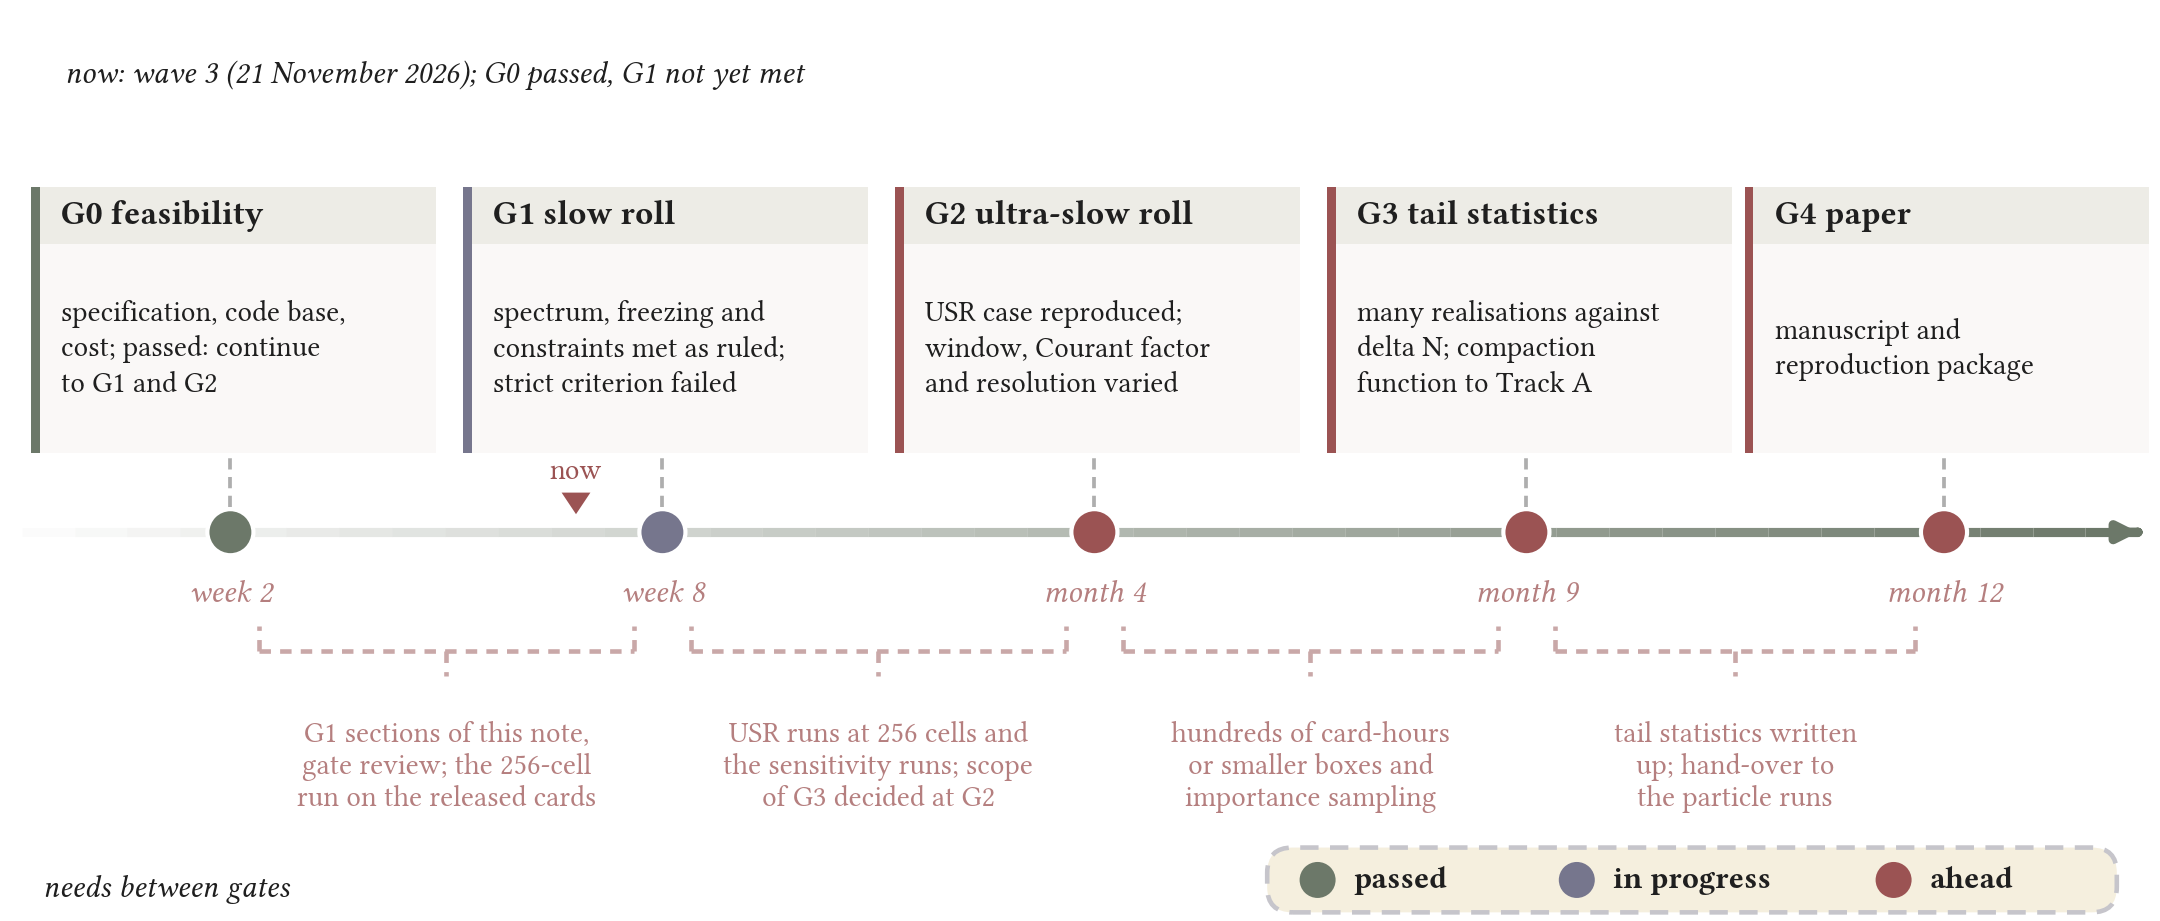
\includegraphics[width=0.92\textwidth]{schem_timeline}
\caption{Stage timeline of the track. Circles: the five gates at their indicative times (green: passed; slate: in progress; red: ahead). Boxes: what each gate requires and, for the first two, where they stand. Dashed brackets: what the step between two gates needs.}
\label{fig:timeline}
\end{figure*}

\section{The slow-roll reproduction}\label{sec:sr}

The slow-roll case tests the whole calculation where linear theory knows the answer for every mode. Once a mode has crossed the window, the curvature perturbation evolved with the full metric must equal the linear mode function times the window and the Gaussian number of its wave vector, and a few e-folds later it must stop evolving. Because the code and the reference share these numbers, one realization decides both statements mode by mode, free of cosmic variance.

\subsection{Runs and analysis}\label{sec:runs}

Two families of runs evolve the quadratic potential for eight e-folds from the initial slice at $N_*$ on periodic lattices. In the set-up of Ref.~\cite{Launay:2025sinr} the noise cutoff grows with the lattice, $k_\mathrm{max}=(N/4)\,\Delta k$ for $N$ cells per side, so the shortest noise wavelength always spans four cells; the run with $256$ cells per side reproduces the published case, and companions with $64^3$ and $128^3$ cells share its cutoff in cells. The convergence ladder fixes the modes instead, $k_\mathrm{max}=8\,\Delta k$, on lattices of $32^3$ to $256^3$ cells, so that one physical solution is resolved ever more finely. Every lattice also runs with all sources reversed in sign, and the lattices up to $128^3$ cells with the amplitude halved, always with the same Gaussian numbers. With the amplitude scale $\lambda$ of the noise (one in the production runs), these mirrored pairs separate the parts of any quantity that are odd and even in $\lambda$. A negative control reverses the kick to the field momentum alone, which violates the constraints at first order by construction.

Figure~\ref{fig:dataflow} shows how the results of this section arise. The case generator of the code writes the background and the mode functions at $N_*$ for every lattice shell, and the track checks them against its own Mukhanov--Sasaki integration. The run dumps the fields, the metric and the constraints, and records box means and constraint ratios at every step. The analysis reconstructs the comoving curvature perturbation $\mathcal{R}^\mathrm{NR}_{\bm n}$ of every lattice mode $\bm k=\bm n\,\Delta k$ from the conformal factor, the trace-free conformal metric and the field, with the extraction factors corrected in Ref.~\cite{Launay:2026thesis}. It compares the result with the linear reference $\mathcal{R}^\mathrm{lin}_{\bm n}=W_k\mathcal{R}_k\alpha_{\bm n}$, whose Gaussian numbers come from an independent implementation of the generator. The criteria are functions of the deviation and of the relative power of each mode,
\begin{equation}\label{eq:Dn}
D_{\bm n}=\left|\frac{\mathcal{R}^\mathrm{NR}_{\bm n}}{\mathcal{R}^\mathrm{lin}_{\bm n}}-1\right|,\qquad
Q_{\bm n}=\frac{|\mathcal{R}^\mathrm{NR}_{\bm n}|^2}{|\mathcal{R}^\mathrm{lin}_{\bm n}|^2}.
\end{equation}
A verifier with its own reader, random numbers, background, mode functions and extraction recomputed the criteria of this section and the next from the raw dumps and confirmed each verdict. Appendix~\ref{app:ledger} gives every number with its run.

\begin{figure*}
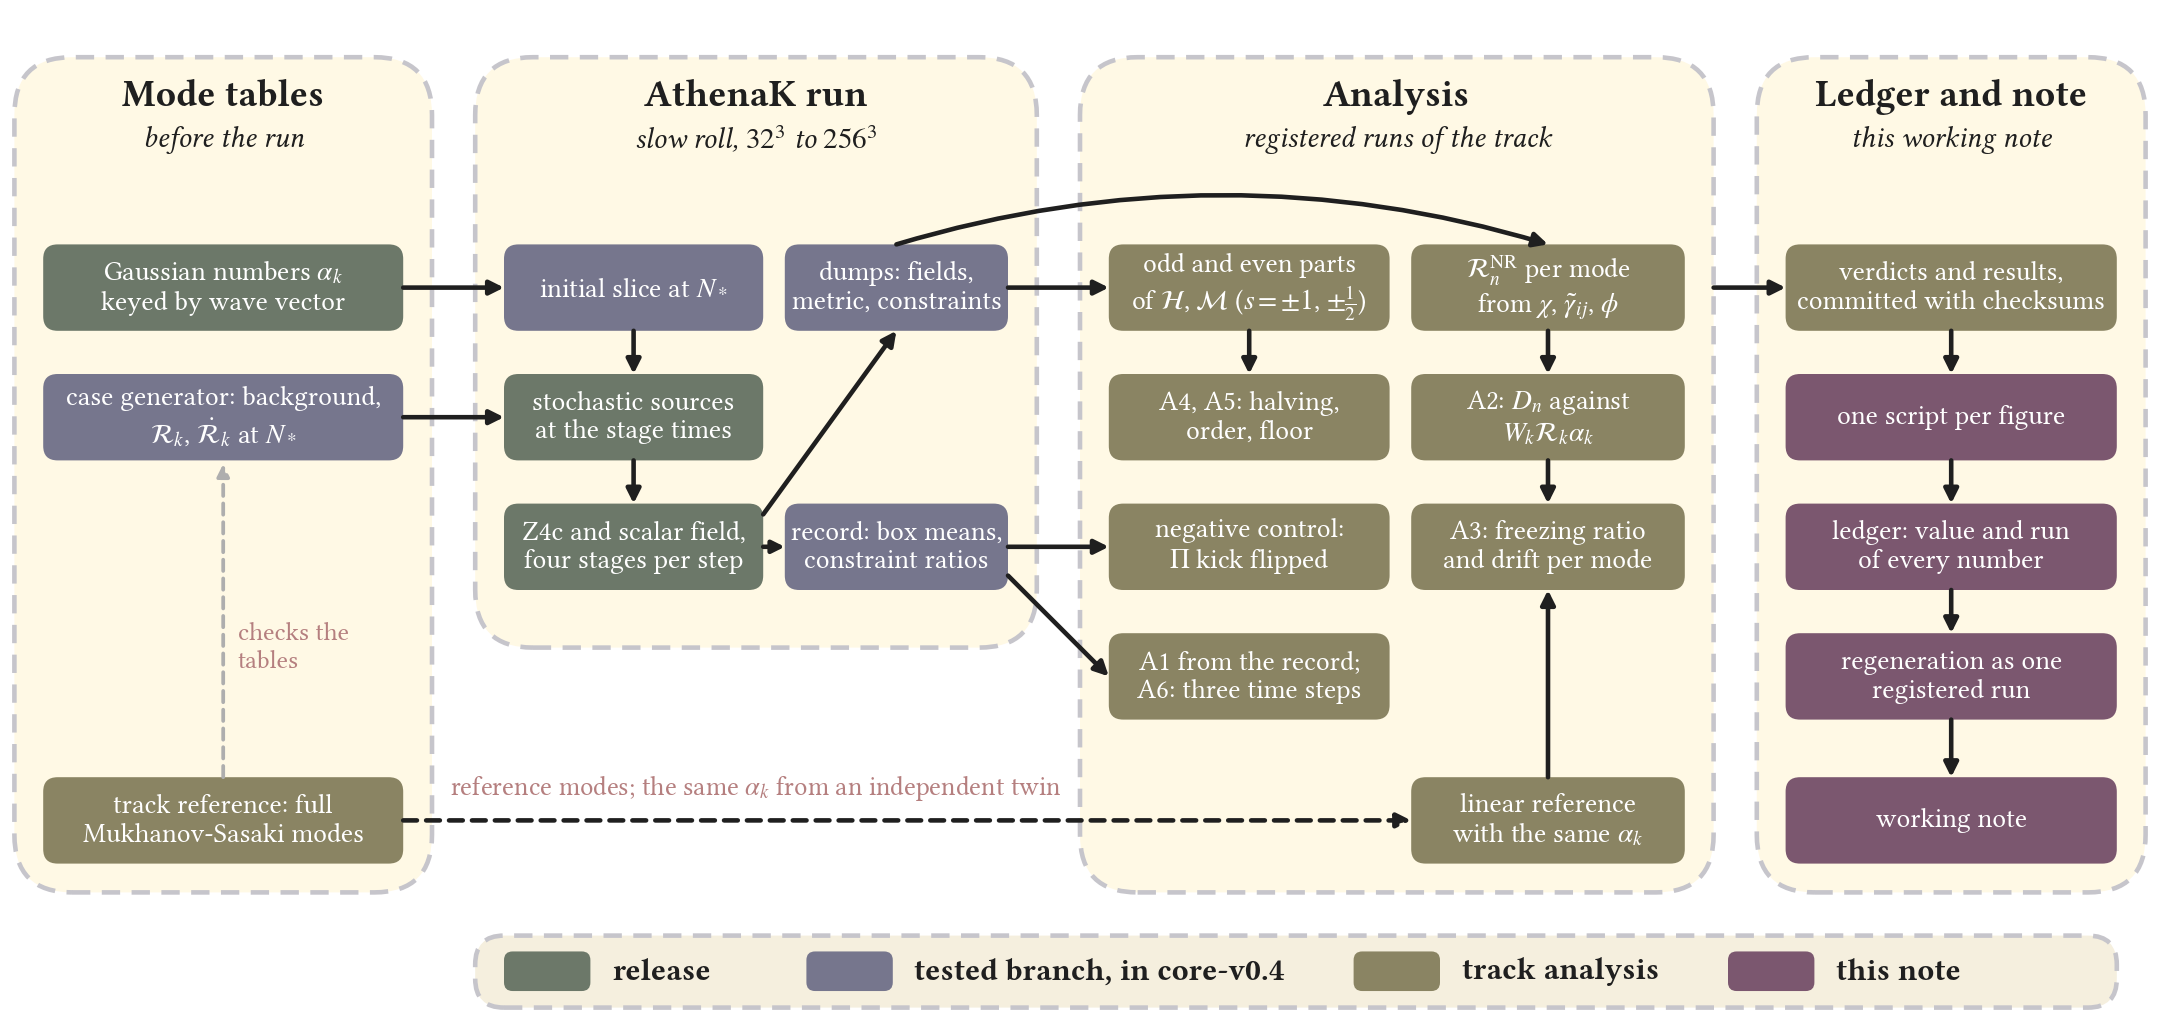
\includegraphics[width=0.96\textwidth]{schem_dataflow}
\caption{Data flow of the slow-roll reproduction, from the mode tables written before a run, through the run in AthenaK and the registered analyses of the track, to the ledger and the figures of this note. Colours mark the parts of the released code, the parts of the tested development state that the release of the code now contains, the track's analysis, and this note; dashed: the independent reference path.}
\label{fig:dataflow}
\end{figure*}

\subsection{Background and amplitude of every mode}\label{sec:a2}

The box means of the field, its momentum and the trace of the extrinsic curvature follow the Friedmann reference close to rounding error on every lattice (A1), and the number of e-folds measured from the mean conformal factor converges at the fourth order of the time integrator. Figure~\ref{fig:modes}(a) shows the deviation of every mode at the end of the run. In the convergence ladder all modes up to the cutoff lie far below the tolerance of A2. Their deviation falls from $32^3$ to $64^3$ cells and then settles at a level independent of the resolution, which we attribute to the part of the curvature perturbation of second order in the noise; a mirrored pair that also dumps the metric would separate it. In the paper's set-up the deviation grows steeply toward the cutoff: this is the dispersion of the sixth-order stencils at four cells per wavelength. The modes up to half the cutoff, which A2 judges, stay far inside the tolerance. Panel (b) follows the largest deviation inside the window: it rises while modes enter and stays flat once the window has passed. The continuum mode function is the reference the code follows, because each mode enters the lattice through the window from the code's continuum mode function; a reference with the wave number of the difference stencil fits worse. The code project points out that this comparison may have used the symbol of the second-order stencil, which remains to be checked. Averaged over shells, with the Gaussian numbers divided out, the power spectrum follows the reference and exceeds the slow-roll formula at crossing by the slow-roll correction that the full Mukhanov--Sasaki solution carries as well.

\begin{figure*}
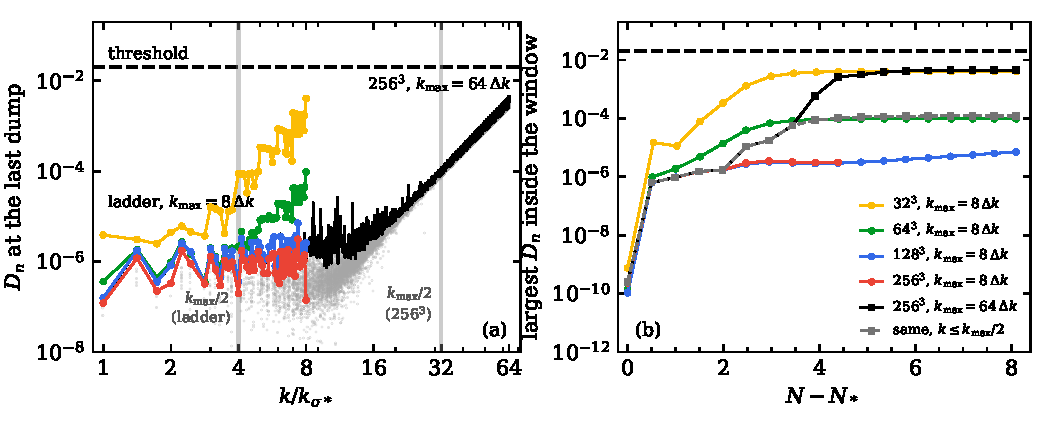
\includegraphics[width=\textwidth]{fig_sr_modes}
\caption{Deviation of the evolved curvature perturbation from linear theory, mode by mode. (a) $D_{\bm n}$ at the end of the run against the wave number in units of the window scale at the start: grey, every mode of the $256^3$ run in the paper's set-up, black, their maximum per shell; coloured, the maxima per shell of the convergence ladder. Vertical lines: half the cutoff of each set-up; dashed: tolerance of A2. (b) Largest $D_{\bm n}$ among the modes inside the window against the e-folds since the start.}
\label{fig:modes}
\end{figure*}

\subsection{Freezing of super-horizon modes in the code}\label{sec:a3}

Figure~\ref{fig:srfreezing} applies the freezing criterion to the $256^3$ run. Every mode that left the window at least six e-folds before the end keeps its power, from four e-folds after crossing to the end, within a tiny fraction of the tolerance of the ratio that the full Mukhanov--Sasaki solution gives (A3), and its residual drift equals that of the full solution, the slow growth of the slow-roll power, to the precision of the fit. The deformed equation of a lattice on a fixed Friedmann background, evaluated for the same shells, loses power at the rate of the decay law of Sec.~\ref{sec:criteria}, far faster than the code drifts. The code therefore freezes the curvature perturbation, and the lattice without metric perturbations is excluded by a wide margin. The rungs of the convergence ladder give the same result.

\begin{figure*}
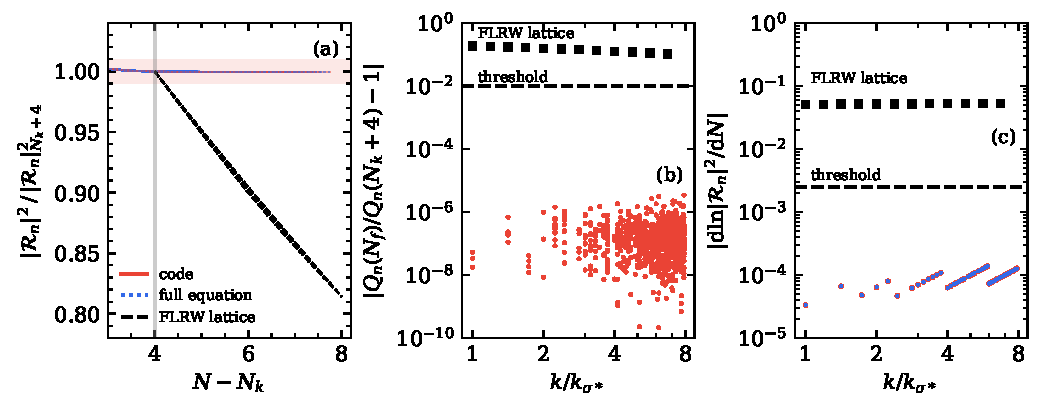
\includegraphics[width=\textwidth]{fig_sr_freezing}
\caption{Freezing of super-horizon modes in the $256^3$ run. (a) Power of sixty randomly chosen modes relative to its value four e-folds after crossing: code (red), full Mukhanov--Sasaki solution (blue dotted), and the deformed equation of a lattice on a fixed background (dashed); band: tolerance of A3. (b) Change of $Q_{\bm n}$ between four e-folds after crossing and the end, per mode; squares: the deformed equation. (c) Drift of the power per e-fold.}
\label{fig:srfreezing}
\end{figure*}

\subsection{Order in time}\label{sec:a6}

With the Courant factor halved twice at $32^3$ cells, the differences between successive runs fall at the fourth order of the integrator throughout the run (A6, Fig.~\ref{fig:order}), for the curvature perturbation of every mode, for the perturbations of the field, the conformal factor and the extrinsic curvature, and for the mean conformal factor. At the Courant factor of the production runs the time error of the curvature perturbation lies far below the tolerance of A2. The deviation of the highest shells, and the first-order part of the constraints during the late entry (Sec.~\ref{sec:constraints}), are the same at all three Courant factors: both are spatial truncation errors.

\begin{figure*}
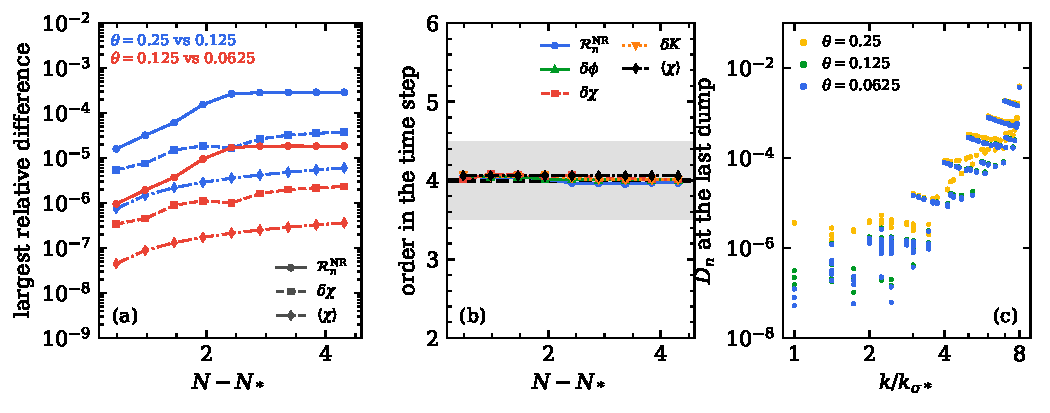
\includegraphics[width=\textwidth]{fig_sr_order}
\caption{Order in time at $32^3$ cells in the convergence set-up. (a) Largest relative difference between runs at Courant factors $\theta$ and $\theta/2$: curvature perturbation per mode, perturbation of the conformal factor $\chi$, and its box mean. (b) Order of convergence from the three runs; band: the range accepted by A6. (c) $D_{\bm n}$ at the end of the run for the three Courant factors.}
\label{fig:order}
\end{figure*}

\section{Constraints}\label{sec:constraints}

The noise enters the momentum of the field and the extrinsic curvature and leaves the metric and the conformal factor unchanged, so the constraints hold only up to terms of second order in the noise (Sec.~\ref{sec:sources}). The Hamiltonian and momentum constraints test whether the code keeps this property, and the reproduction's criterion A4 asked that their violation be of second order while the modes enter the window.

\subsection{The record}\label{sec:record}

The code records at every step the box means of $|\Ham|$ and $|\Mom_i|$ divided by those of their term magnitudes $[\Ham]$ and $[\Mom]$, the sums of the absolute values of the terms of each constraint. In the paper's set-up the Hamiltonian ratio stays close to the level the source paper reports and the momentum ratio stays small; in the negative control the Hamiltonian ratio rises by several orders of magnitude and the momentum ratio becomes a sizeable fraction of one, as in the source paper. The record ratios, however, measure no order in the noise. The Hamiltonian ratio contains a uniform residual of the time integration of the background, which converges at the fourth order of the integrator and is independent of the noise amplitude, and the momentum magnitude $[\Mom]$ is itself of first order in the amplitude.

\subsection{Parts odd and even in the noise amplitude}\label{sec:split}

A mirrored pair of runs with amplitudes $\pm\lambda$ separates each constraint into
\begin{equation}\label{eq:split}
\begin{aligned}
\Ham_\mathrm{odd}&=\tfrac12\left[\Ham(\lambda)-\Ham(-\lambda)\right],\\
\Ham_\mathrm{even}&=\tfrac12\left[\Ham(\lambda)+\Ham(-\lambda)\right],
\end{aligned}
\end{equation}
the parts of odd and of even order in $\lambda$, and the same for $\Mom_i$. Figure~\ref{fig:constraints}(a) shows their root mean square over the box. The even part is the physical second-order violation. It falls by the factor four when the amplitude is halved (panel b), and it is the same at every resolution: it agrees closely between $64^3$ and $128^3$ cells, and, in the convergence set-up, between $128^3$ and $256^3$ cells once each run's floor is removed. The odd part falls by the factor two when the amplitude is halved, so it is of first order. It is small at the start and rises steeply once shells with fewer than eight cells per wavelength enter the window, which in the paper's set-up happens $\ln(N/8)$ e-folds after $N_*$; from then on it exceeds the even part by a large factor at $32^3$ to $128^3$ cells. At $256^3$ cells the last dump at which both runs of the pair share the time comes shortly before the top shell enters, and there the odd part has also risen above the even part. In the convergence set-up the odd part converges at fifth to sixth order until it reaches a floor, and from $128^3$ cells on it stays below the even part. The floor is the part that is independent of the amplitude; it grows with the number of cells, and we attribute it to rounding.

\begin{figure*}
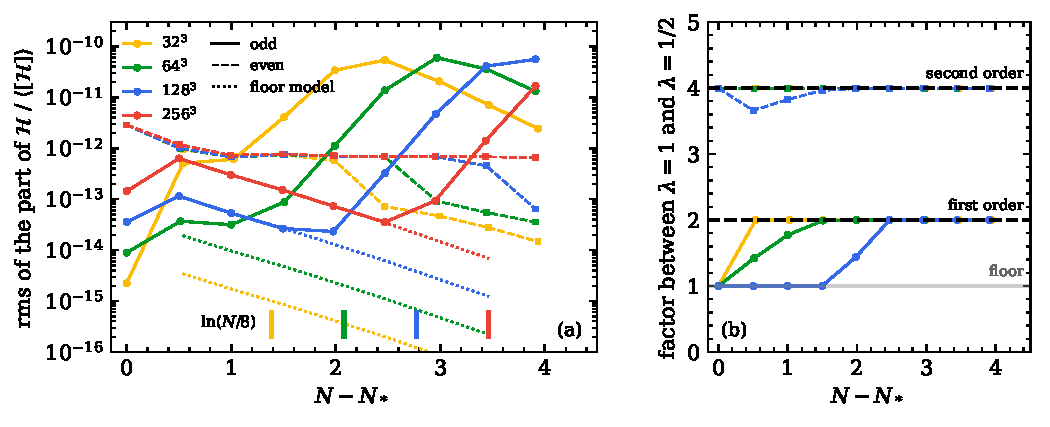
\includegraphics[width=\textwidth]{fig_sr_constraints}
\caption{Hamiltonian constraint of the slow-roll runs split into parts odd (solid) and even (dashed) in the noise amplitude, in the paper's set-up for $32^3$ to $256^3$ cells. (a) Root mean square over the box of each part, divided by the box mean of the term magnitude; ticks: $\ln(N/8)$ e-folds after the start; dotted: the model of the amplitude-independent floor of the odd part. (b) Factor by which each part falls when the amplitude is halved: two at first order, four at second order, one for the floor.}
\label{fig:constraints}
\end{figure*}

\subsection{The criterion}\label{sec:a4}

The strict criterion A4 therefore fails in the set-up of the source paper at every resolution we ran: from $\ln(N/8)$ e-folds after the start the constraint violation is dominated by a part of first order in the noise. It holds in the convergence set-up from $128^3$ cells on. The failure stays on record. The first-order part is a discretization error of the code, since it converges with resolution, while the record ratios mix it with the physical violation and with the residual of the time integration. The program's ruling after the verifier's report adopted the reworded criterion A4$'$, which judges the two parts separately. The even part must fall by four under halving and agree between the two finest resolutions above the floor. The odd part must fall by two under halving and converge at the order of the convergence criterion A5, and it may exceed the even part while the shells with fewer than eight cells per wavelength enter. The record ratios must stay near the levels of the source paper, and the maxima over the entry of the first-order parts of the negative control and of the proper run must lie far apart. The floor in A4$'$ and in A5 is the part independent of the amplitude; this operational definition was fixed after the data were seen. The runs pass A4$'$. Its last clause holds for the maxima over the entry; pointwise, at the end of the entry, the separation between control and proper run is much smaller (Appendix~\ref{app:ledger}).

The code project traced the first-order part to the discrete form of the contracted Bianchi identity, which keeps the constraints satisfied in the continuum evolution. Linearized about the homogeneous background, a first difference acts on a Fourier mode as $iq_a$ and a second difference as $-\kappa_a$, and the constraints of the mesh are driven by the linear solution times
\begin{equation}\label{eq:mu}
\mu_a=\kappa_a-q_a^2,
\end{equation}
the mismatch between the second difference and the first difference applied twice. The mismatch is largest at four cells per wavelength, falls at the sixth order of the stencils, and is independent of the time step. A linear model of the code's difference equations, with the stages of the integrator, reproduces the measured odd parts of the convergence ladder at $32^3$ cells at every dump. By this model the strict criterion would hold at $256^3$ cells only with a noise cutoff well below the published one (Appendix~\ref{app:ledger}). The explanation awaits an independent check by the track. \pending{the check of this explanation with the symbols of the stencils and with a halved pair in the convergence set-up.}

\section{Validation, reproducibility and cost}\label{sec:validation}

\subsection{The analysis}\label{sec:analysis}

The analysis was validated before it judged the code. On synthetic fields with known answers it passes all its tests; among them, the curvature perturbation reconstructed from a metric perturbation of known amplitude carries an error of second order in the amplitude, and leaving out the metric term fails by a wide margin. Its reader of the dumps agrees bit for bit with the code's own reader, and at the start of a run the reconstructed curvature perturbation equals the linear reference to rounding error. The runs also settled the coefficient of the anisotropic term of the extraction, which the source papers print in mutually inconsistent forms: with the factor one quarter of Ref.~\cite{Launay:2026thesis} the deviation of the $32^3$ rung lies far below the tolerance, and the other printed forms or the omission of the term deviate many times more. The verifier's independent pipeline reproduced the track's numbers and every verdict; its disagreements concerned dumps of a pair taken at different times and maxima quoted too low in one summary, and this note uses the corrected values.

\subsection{Reproducibility}\label{sec:reproducibility}

The noise is a deterministic function of its keys. The source fields are bit-identical for one, eight and sixty-four MeshBlocks and through a restart, on processors and on a card, and the card differs from the processors by rounding only (A7). The executable of the slow-roll runs gives bit-identical values of all variables for one and eight MeshBlocks and through a restart, and the released processor build reproduces the mirrored $32^3$ pair word for word. The released card build and runs on several processes remain to be compared.

\subsection{Cost of one realization}\label{sec:srcost}

One realization of the slow-roll case at $256^3$ cells, eight e-folds at Courant factor $\theta=0.25$ on one card, costs slightly less than the range extrapolated at the feasibility gate from the throughput at $128^3$ (Sec.~\ref{sec:cost}), and far below the downgrade threshold. The measured cost replaces the extrapolation.

\section{What is open}\label{sec:open}

At the slow-roll gate the spectrum and the freezing pass with wide margins, and the constraints pass the criterion in force after the ruling, with the strict criterion failed on record. The gate itself waits for these sections of the note and for their independent review, which includes a recomputation of the ledger of Appendix~\ref{app:ledger}. Further items of the slow-roll case are the $256^3$ run on the released card build; the constraint split of the $256^3$ run after the top shell enters, which needs a partner run to the end; a mirrored pair with metric dumps that separates the floor of the curvature perturbation on the finer rungs; the absolute constraint levels, which lie well below those the source paper states, for a reason still open; and the check of the code project's explanation of the first-order part.

The USR gate needs the inflection case at $256^3$ cells on cards, with the mode tables and the initial slice that the code now provides, and the sensitivity of the results to the window, the Courant factor and the resolution. \pending{first results of the ultra-slow-roll runs.} \pending{sensitivity of the slow-roll results to the window.} Levels 1 and 2 of the stochastic backreaction, a slice beyond first order in the constraints, and the hand-over to the particle runs of the primordial-black-hole track come later (Fig.~\ref{fig:architecture}). Of the items of the feasibility gate, the validation of the noise generator at the base size on a card is done, the reference forms the window increment as the code does, and the cost is measured; the key statements of the references still wait to enter the knowledge base of the program, and the end-of-inflation statistics after USR and the importance sampling of the phase-space solver still await an independent re-check.

\section{Summary}\label{sec:summary}

A reproduction of stochastic inflation in numerical relativity can be judged on a single realization, because the code and its reference share the Gaussian number of every wave vector. In slow roll the code passes this test: every resolved mode follows linear theory, and every super-horizon mode freezes where the full Mukhanov--Sasaki equation freezes, while a background lattice without metric perturbations visibly fails. The constraints reveal a property of the difference stencils that a criterion phrased in record ratios hides: when the shortest noise modes enter with four cells per wavelength, the stencils violate the constraints at first order in the noise, above the physical second-order violation, and this part converges with resolution. Judged by its parts odd and even in the noise, the code behaves as the continuum equations say. The separate-universe reference must use a narrow window, because the coarse-graining of the numerical-relativity runs inflates the delta-N variance by modes that still carry gradients. The noise of the code is a deterministic function of its keys, so it is reproducible across resolutions, decompositions of the mesh into blocks and restarts by construction, and the tests confirm it. The open question for the next gate is physical: whether the curvature perturbation evolved with full metric backreaction follows linear theory through the transitions into and out of ultra-slow roll, where the separate-universe approximation is in doubt.

\begin{acknowledgments}
This note, its figures and the calculations behind them were produced by large-language-model agents (Claude) working in the program's repository under human direction. Third-party paper sources were read in the program's local store, which keeps them private.
\end{acknowledgments}

\appendix

\section{Parameters}\label{app:parameters}

Table~\ref{tab:parameters} lists the parameters of the two test cases. The printed parameters are those of Ref.~\cite{Launay:2025sinr}; the derived ones come from the track's reference integrator, and an independent integrator agrees with them.

\begin{table*}
\caption{\label{tab:parameters}Parameters of the two test cases.}
\begin{ruledtabular}
\footnotesize
\begin{tabular}{lll}
 & slow roll & ultra-slow roll \\
\hline
potential & $\tfrac12 m^2\phi^2$ & inflection form \\
parameters of the source & $\epsilon_1=0.01$, $\epsilon_2=-0.02$ & $\Lambda=1.86\times10^{-6}$, $v=0.198\,M_\mathrm{Pl}$ \\
 & $H_0=10^{-5}M_\mathrm{Pl}$ & $\phi_0=-1.2\,M_\mathrm{Pl}$ \\
derived & $\phi_0=-14.0950\,M_\mathrm{Pl}$ & $H_0=9.5902\times10^{-6}M_\mathrm{Pl}$ \\
 & $m=1.73494\times10^{-6}M_\mathrm{Pl}$ & $\mathrm{d}\phi/\mathrm{d}N=0.102682\,M_\mathrm{Pl}$ \\
$N_*-N_0$, $N_f-N_*$ & $5$, $8$ & $3$, $10$ \\
lattice & \multicolumn{2}{l}{$256^3$ cells, $L\,k_{\sigma*}=2\pi$, $k_\mathrm{max}=64\,\Delta k$} \\
window & \multicolumn{2}{l}{$\tanh$ profile, steepness $s=5$, $\sigma=1$} \\
gauge & \multicolumn{2}{l}{geodesic slicing, zero shift, undamped} \\
Courant factor & \multicolumn{2}{l}{$0.25$; tests at $0.125$, $0.0625$} \\
noise coefficients & \multicolumn{2}{l}{Friedmann background; box means as a variant} \\
\end{tabular}
\end{ruledtabular}
\end{table*}


\section{Corrections to the source papers}\label{app:errata}

Table~\ref{tab:errata} lists the corrections found while writing the specification. Each was checked by a registered calculation or an independent derivation; the locators are in the track's specification.

\begin{table*}
\caption{\label{tab:errata}Corrections to the source papers.}
\begin{ruledtabular}
\footnotesize
\begin{tabular}{p{0.19\textwidth}p{0.42\textwidth}p{0.27\textwidth}}
Item & Correction & Check \\
\hline
Momentum of the initial slice \cite{Launay:2025bd} & the printed term in the lapse potential vanishes in geodesic slicing; the slice needs $-\sqrt{2\epsilon_1}\Mpl H\Psi_B$ & linearized Hamiltonian constraint symbolic: nonzero printed, zero corrected; re-derived from the gauge dictionary \\
Random-draw normalization \cite{Launay:2025bd,Launay:2026thesis} & field $=L^{-3/2}$ times the inverse transform of amplitude times draw; the two printed prefactors are mutually inconsistent and give too much power by powers of $2\pi$ & measured shell power against the target \\
Importance-sampling weight \cite{Jackson:2022is} & sign of the exponent: with the printed sign the expected weight is far from unity & expected weight unity within errors \\
Leading pole \cite{Jackson:2022is} & for a finite ultraviolet boundary the leading pole is the lowest eigenvalue of the first-passage problem, and the closed form is smooth through the stated value & closed form against the Sturm--Liouville eigenvalues \\
Friedmann equation \cite{Launay:2025sinr} & denominator lacks $3\Mpl^2$; the ``very shallow maximum'' is an exact stationary inflection point at $\phi=-\sqrt2\,v$ & reading; double root of the potential's slope \\
USR interval \cite{Launay:2025sinr} & the text places USR about one e-fold later than its own background figure & two independent background integrators \\
Extraction of $\mathcal{R}^\mathrm{NR}$ \cite{Launay:2025bd} & the printed factors of the anisotropic metric term are wrong; the factor is one quarter, as corrected in Ref.~\cite{Launay:2026thesis} & per-mode deviation of the slow-roll runs with each factor; re-derived from the dictionary \\
\end{tabular}
\end{ruledtabular}
\end{table*}

\section{Numerical ledger}\label{app:ledger}

Tables~\ref{tab:ledger} and \ref{tab:ledgerG1} list the numbers behind the statements and figures of this note with the registered runs that produced them, Table~\ref{tab:ledger} for the feasibility gate and Table~\ref{tab:ledgerG1} for the slow-roll reproduction. The figures and the tables are made by one registered run of the note's scripts, which check each input against the checksum its run records; a few numbers of the verifier, of a check of the released build and of the code project are read at their lines in the reports that state them. The same run recomputes the numbers printed in the track's documents from the run outputs: they agree to their printed digits, except the assumed overhead of the field and the sources and the cost per realization that follows from it, which the measured throughput replaces (Sec.~\ref{sec:cost}); the last printed digit of the first slow-roll parameter at the start of the USR case, where the two independent integrators differ; and two maxima of the background box means in one summary of the slow-roll runs, which understate the computed values.

\begin{table*}
\caption{\label{tab:ledger}Numerical ledger: the numbers behind the statements and figures of this note, each with the registered run that produced it.}
\begin{ruledtabular}
\footnotesize
\begin{tabular}{p{0.56\textwidth}p{0.26\textwidth}p{0.08\textwidth}}
Quantity & Value & Run \\
\hline
Background, SR: first slow-roll parameter at the start & $0.01111$ & R1 \\
Background, SR: first slow-roll parameter at the end & $0.0135$ & R1 \\
Background, USR: first slow-roll parameter at the start & $0.01316$ & R1 \\
Background, USR: interval with $\epsilon_2>3$ (e-folds after the start) & $2.524$--$6.550$ & R2 \\
Background, USR: minimum of the first slow-roll parameter & $9.716\times10^{-13}$ & R1 \\
Freezing, SR: full power at the end over the slow-roll estimate at crossing & $1.0104$--$1.0121$ & R1 \\
Freezing, SR: drift of $\ln\Delta_\mathcal{R}$ per e-fold, full, from $N_k+3$ & $-0.00189$ to $-0.000253$ & R1 \\
Freezing, SR: drift per e-fold, deformed & $-0.0552$ to $-0.0509$ & R1 \\
Freezing, SR: deformed over full power at the end, $k=\Delta k$ and $64\,\Delta k$ & $0.654$, $0.794$ & R1 \\
Freezing, USR: deformed over full power at the end, $k=\Delta k$, $4\,\Delta k$ & $8.40$, $1.180$ & R1 \\
Freezing, USR: full power at the end, $k=64\,\Delta k$ & $1.0168$ & R1 \\
Freezing, independent check: SR slopes full, deformed; $-4\epsilon_1$ & $-0.00058$, $-0.0519$; $-0.0513$ & R2 \\
$\delta N$, SR: linear variance of the band & $3.9248\times10^{-10}$ & R3 \\
$\delta N$, USR: linear variance of the band & $0.79884$ & R4 \\
$\delta N$: lattice sum over continuum, SR, USR & $1.0805$, $0.9997$ & R3, R4 \\
$\delta N$, SR: variance over linear at $\sigma=0.01,\,0.1,\,1$ & $0.9981$, $1.0050$, $1.4492$ & R3 \\
$\delta N$, USR: variance over linear at $\sigma=0.01,\,0.1,\,1$ & $1.0001$, $1.0055$, $1.4233$ & R4 \\
$\delta N$: skewness at $\sigma=0.01$, SR, USR & $0.003$, $0.038$ & R3, R4 \\
Noise: reconstruction from the keys, frozen, Markov-step, Markov-tanh (tolerance $10^{-11}$) & $4.1\times10^{-14}$, $2.4\times10^{-15}$, $1.07\times10^{-10}$ & R5 \\
Noise: frozen scheme, $N$ against $2N$ & $2.4\times10^{-15}$ & R5 \\
Cost: Z4c; with field; with sources (zone-cycles per second, $128^3$) & $1.98\times10^{7}$; $1.39\times10^{7}$; $1.2\times10^{7}$ & R7 \\
Cost: overhead of field and sources over Z4c, assumed; measured & $0.15$; $0.65$ & R6, R7 \\
Cost, SR $256^3$: steps; card-hours model; measured throughput & $1304$; $0.41$; $0.57$--$0.71$ & R6, R7 \\
Cost, USR $256^3$: steps; card-hours model; measured throughput & $1630$; $0.51$; $0.71$--$0.88$ & R6, R7 \\
Cost: memory of a $256^3$ run (GB) & $19.7$ & R6 \\
\hline
\multicolumn{3}{l}{Registered runs:} \\
\multicolumn{3}{l}{R1\quad\texttt{E-stoch-inf-20261115-122806-ef0d039}\quad background and mode functions, full and deformed} \\
\multicolumn{3}{l}{R2\quad\texttt{E-20261115-135532-3f958a1}\quad independent background, freezing and delta-N checks} \\
\multicolumn{3}{l}{R3\quad\texttt{E-stoch-inf-20261115-130139-176cdd6}\quad stochastic delta N, slow roll} \\
\multicolumn{3}{l}{R4\quad\texttt{E-stoch-inf-20261115-130137-176cdd6}\quad stochastic delta N, ultra-slow roll} \\
\multicolumn{3}{l}{R5\quad\texttt{E-20261115-140502-2957846}\quad validation of the code's noise generator} \\
\multicolumn{3}{l}{R6\quad\texttt{E-20261115-140116-87c1cc5}\quad cost model and synthesis operation counts} \\
\multicolumn{3}{l}{R7\quad\texttt{core-20261115-143907-cea4c86}\quad measured card throughput of the code (core)} \\
\end{tabular}
\end{ruledtabular}
\end{table*}


\begin{table*}
\caption{\label{tab:ledgerG1}Numerical ledger of the slow-roll reproduction, criteria A1 to A6: each number with the registered run that produced it (runs listed in Table~\ref{tab:ledgerG1b}, R1 in Table~\ref{tab:ledger}).}
\begin{ruledtabular}
\footnotesize
\begin{tabular}{p{0.56\textwidth}p{0.27\textwidth}p{0.08\textwidth}}
Quantity & Value & Run \\
\hline
A1: box means of $\phi$, $\Pi$, $K$ against the Friedmann reference, largest over the rungs & $2.0\times10^{-12}$, $8.6\times10^{-12}$, $3.6\times10^{-12}$ & R9 \\
A1: e-folds from $\langle\chi\rangle$ after 8.1 e-folds, $32^3$, $64^3$, $128^3$ & $5.5\times10^{-6}$, $3.3\times10^{-7}$, $2.0\times10^{-8}$ & R9 \\
A2: largest $D_n$ for $k\leq k_\mathrm{max}/2$, ladder $32^3$, $64^3$, $128^3$, $256^3$ & $8.8\times10^{-5}$, $2.7\times10^{-6}$, $2.5\times10^{-6}$, $1.7\times10^{-6}$ & R9 \\
A2: the same in the paper's set-up, $64^3$, $128^3$, $256^3$ & $9.7\times10^{-5}$, $9.9\times10^{-5}$, $1.21\times10^{-4}$ & R9 \\
A2: modes of the $256^3$ run, all and with $k\leq k_\mathrm{max}/2$ & $548958$, $68532$ & R9 \\
A2: largest $D_n$ over all modes, ladder $32^3$, $64^3$, $128^3$ & $4.08\times10^{-3}$, $9.65\times10^{-5}$, $7.09\times10^{-6}$ & R9 \\
A2: $256^3$ against a reference with the stencil's wave number & $6.16\times10^{-3}$ & R9 \\
Spectrum: shell ratio against the reference with the same $\alpha_k$, largest over the rungs & $1.9\times10^{-4}$ & R9 \\
Spectrum: linear power over the slow-roll formula, $k\leq7\,k_{\sigma*}$ & $1.0104$--$1.0109$ & R9 \\
A3: modes with $N_f-N_k\geq6$ per rung & $1051$ & R9 \\
A3: largest $|Q_n(N_f)/Q_n(N_k+4)-1|$ over the rungs & $4.6\times10^{-6}$ & R9 \\
A3: largest drift of $\ln|\mathcal{R}_n|^2$ per e-fold, range over the rungs & $1.379\times10^{-4}$--$1.405\times10^{-4}$ & R9 \\
A3: drift of the code minus that of the full equation, largest & $1.75\times10^{-6}$ & R9 \\
A3: drift of the FLRW lattice for the same shells; over the largest drift of the code & $0.0513$--$0.0527$; $365$ & R1, R9 \\
A4: largest odd over even part of $\mathcal{H}$ at dumps where both runs of the pair share the time, paper set-up, $32^3$, $64^3$, $128^3$, $256^3$ & $745$, $655$, $869$, $25$ & R9 \\
A4: e-folds of these maxima; last time-matched dump of the $256^3$ pair & $2.47$, $2.97$, $3.91$, $3.91$; $3.91$ & R9 \\
A4: first dump with odd above even part (e-folds); $\ln(N/8)$, same lattices & $1.51$, $1.99$, $2.96$, $3.44$; $1.39$, $2.08$, $2.77$, $3.47$ & R10 \\
A4: largest record $\langle|\mathcal{H}|/[\mathcal{H}]\rangle$; $\langle|\mathcal{M}|/[\mathcal{M}]\rangle$, paper set-up & $5.1\times10^{-11}$; $3.8\times10^{-4}$ & R9 \\
A4: halving factors at $32^3$, odd part; even part & $1.9999$--$2.0000$; $3.991$--$4.000$ & R10 \\
A4: largest odd over even part, convergence set-up, $64^3$, $128^3$, $256^3$ & $15.4$, $0.27$, $0.53$ & R9 \\
Negative control: record $\mathcal{H}$ over the proper run, range of the maxima; $\langle|\mathcal{M}|/[\mathcal{M}]\rangle$ & $4.0\times10^{4}$--$1.5\times10^{5}$; $0.20$--$0.22$ & R9 \\
A5: order of the odd part before the floor, $32^3\to64^3\to128^3$, $\mathcal{H}$; $\mathcal{M}$ & $4.20$--$5.82$; $5.55$--$5.91$ & R10 \\
Floor: growth with the cells per side, exponent for $\mathcal{H}$; $\mathcal{M}$ & $2.48$; $2.63$ & R10 \\
Floor: odd part of $\mathcal{H}$ at $256^3$, first and last dump of the comparison & $6.0\times10^{-13}$, $6.9\times10^{-15}$ & R10 \\
Even part: $64^3$ against $128^3$, largest relative difference & $0.022$ & R10 \\
Record $\langle|\mathcal{H}|/[\mathcal{H}]\rangle$ at $N_f$, $32^3$, $64^3$, $128^3$ & $3.12\times10^{-12}$, $1.83\times10^{-13}$, $1.12\times10^{-14}$ & R9 \\
A6: orders of the differences between Courant factors & $3.93$--$4.08$ & R11 \\
A6: largest difference of $\mathcal{R}^\mathrm{NR}_n$ between $\theta=0.25$ and $0.125$ & $2.9\times10^{-4}$ & R11 \\
A6: largest $D_n$ of the top shells at $\theta=0.25$, $0.125$, $0.0625$ & $3.97\times10^{-3}$, $3.75\times10^{-3}$, $3.74\times10^{-3}$ & R11 \\
A6: odd part of $\mathcal{H}$ in the late entry, largest change per halving of $\theta$ & $0.041$ & R11 \\
A6: order of the uniform residual of $\mathcal{H}$ & $4.10$ & R11 \\
\end{tabular}
\end{ruledtabular}
\end{table*}

\begin{table*}
\caption{\label{tab:ledgerG1b}Numerical ledger of the slow-roll reproduction, continued: reproducibility, analysis, cost, the verifier and the code project; the registered runs of both parts.}
\begin{ruledtabular}
\footnotesize
\begin{tabular}{p{0.56\textwidth}p{0.27\textwidth}p{0.08\textwidth}}
Quantity & Value & Run \\
\hline
A7: noise for one, eight, sixty-four MeshBlocks; restart on processors, card; card against processors & $0$; $0$, $0$; $2.2\times10^{-15}$ & R16, R18, R17 \\
A7: variables bit-identical between one and eight MeshBlocks and through a restart, the executable of the slow-roll runs at $32^3$ & $22$ of $22$ & V \\
A7: released processor build against the executable of the slow-roll runs, $32^3$ pair: 64-bit words compared; differing & $18.9\times10^{6}$; $0$ & L \\
Analysis: synthetic tests passed & $15$ of $15$ & R13 \\
Analysis: $\mathcal{R}^\mathrm{NR}$ at amplitude $10^{-5}$, error and its slope; without the metric term & $2.35\times10^{-4}$, $0.999$; $0.657$ & R13 \\
Analysis: reader against core's, largest difference; $D_n$ at the start & $0$; $7.5\times10^{-10}$ & R14 \\
Analysis: largest $D_n$ ($32^3$, $k\leq k_\mathrm{max}/2$) with the factor $1/4$, $1/2$, $-1/4$, none & $8.8\times10^{-5}$, $5.2\times10^{-3}$, $0.010$, $5.1\times10^{-3}$ & R15 \\
Cost of one $256^3$ realisation, 8.1 e-folds: card-hours; seconds; steps & $0.503$; $1811$; $1386$ & R12, R9 \\
Cost: seconds per step at $256^3$ on one card & $1.13$--$1.30$ & R9 \\
Verifier: control over proper first-order part, ratio of the maxima over the entry; pointwise at the end of the entry, lowest & $1709$--$1874$; $89$ & V \\
Verifier: even part, $128^3$ against $256^3$ in the convergence set-up after each run's floor is removed (percent) & $0.8$ & V \\
Core: stencil mismatch $\mu/k^2$ at four, eight, sixteen cells per wavelength & $0.110$, $2.6\times10^{-3}$, $4.4\times10^{-5}$ & C \\
Core: largest odd over even part at four cells per wavelength; cells where it falls below one & $692$; $12.7$ & C \\
Core: largest noise cutoff at $256^3$ for second-order constraints & $20\,\Delta k$ & C \\
\hline
\multicolumn{3}{l}{Registered runs:} \\
\multicolumn{3}{l}{R9\quad\texttt{E-20261115-194633-9e04ed8}\quad final analysis of the slow-roll ladder (A1-A5, spectrum, negative control)} \\
\multicolumn{3}{l}{R10\quad\texttt{E-20261119-142713-32c883a}\quad floor analysis of the odd constraint parts (A5, halving, crossing)} \\
\multicolumn{3}{l}{R11\quad\texttt{E-20261119-145230-ff0dff2}\quad temporal order A6 (three Courant factors at $32^3$)} \\
\multicolumn{3}{l}{R12\quad\texttt{E-20261115-172618-f948386}\quad $256^3$ slow-roll run in the paper's set-up on one card (cost)} \\
\multicolumn{3}{l}{R13\quad\texttt{E-20261115-171445-36152c4}\quad synthetic tests of the analysis module} \\
\multicolumn{3}{l}{R14\quad\texttt{E-20261115-172935-ddfade0}\quad reader of the dumps against core's reader} \\
\multicolumn{3}{l}{R15\quad\texttt{E-20261115-174214-74becdd}\quad extraction factor of the anisotropic term of the curvature perturbation} \\
\multicolumn{3}{l}{R16\quad\texttt{E-20261115-180533-24a7781}\quad noise for three MeshBlock layouts on a card} \\
\multicolumn{3}{l}{R17\quad\texttt{E-20261115-184748-9b010fa}\quad card against processors} \\
\multicolumn{3}{l}{R18\quad\texttt{E-20261119-141654-c2a10d1}\quad restart on processors and on a card} \\
\multicolumn{3}{p{0.93\textwidth}}{V\quad the verifier's runs \texttt{E-20261121-030207-fb6f090, -031951-82984f8, -030522-c6907b6, -031049-27cdc06, -031251-c48670d}, its report and the stage status of the gate} \\
\multicolumn{3}{l}{L\quad the lead's check \texttt{E-20261121-064707-77ec326}} \\
\multicolumn{3}{p{0.93\textwidth}}{C\quad core's runs \texttt{core-20261119-151758-51d9a71, -152243-1754ebc, -161111-9d05d14}, its interface text of release core-v0.5} \\
\end{tabular}
\end{ruledtabular}
\end{table*}


\bibliography{references}

\end{document}
